\subsection{Efficient Flight Planning}

Efficient flight planning is a cornerstone of modern \gls{ATM}, particularly as global air traffic continues to grow and demands on limited airspace intensify.
Civil aviation flight plans are developed under \glspl{IFR} and must consider capacity constraints, aircraft performance limitations, and airline preferences.
However, even though flight plans are typically filed about an hour before departure, they are often not executed as planned due to factors such as adverse weather, ground congestion, and delayed arrivals  \cite{Rosenow_2021}.
These disruptions reduce airport efficiency and propagate delays throughout the air traffic network, a phenomenon often referred to as the ripple effect \cite{Ye_2024}.

Traditional \gls{ATM} research has largely focused on tactical-level solutions such as flow management, but there is growing recognition that strategic-level flight planning also plays a crucial role.
The works of Rosenow et al. \cite{Rosenow_2021} and Ye et al. \cite{Ye_2024} offer promising approaches to solving strategic flight planning challenges using optimisation and \gls{AI}.

Rosenow et al. \cite{Rosenow_2021} identify that conventional flight planning still heavily relies on manual processes and heuristic methods that do not fully account for the dynamic and multi-objective nature of the airspace environment.
As a result, suboptimal routes are often chosen, leading to excessive fuel consumption, extended flight times, and increased emissions.
To address this, the authors propose a multi-objective optimisation model that balances multiple goals while maintaining logical route structures and time constraints.
% These goals include minimising fuel use, reducing delays, and maximising airspace utilisation.
The results demonstrate significant potential for \gls{AI}-driven models to improve operational efficiency and environmental sustainability.

Similarly, Ye et al. \cite{Ye_2024} propose a strategic flight planning framework tailored to high-demand, weather-sensitive regions in China.
Their model optimises flight scheduling with two objectives: (1) minimising total departure and arrival time offsets (\gls{FMS}), and (2) reducing strategic operational costs, including ground and airborne components (\gls{FMC}).
Using real-world data from rainy and foggy seasons at \gls{CTU}, \gls{TCZ}, and \gls{LUM}, the model showed that rerouting flights to less congested airports like \gls{LUM} during capacity constraints at \gls{TCZ} is both feasible and cost-effective.
This effectively reduces the decision-making burden on \glspl{ATCO}.

While these models highlight the effectiveness of optimisation in strategic planning, their real-world deployment faces challenges.
Current models are often constrained by limited datasets and simplifications that fail to capture the full complexity of live airspace operations.
As \gls{UAM} begin to integrate into civilian airspace, such as those using vertiports (e.g., \gls{MUC}, Figure \ref{vertiport}), the need for more robust, adaptive, and \gls{AI}-powered optimisation frameworks becomes critical.
Future systems must be capable of dynamically coordinating mixed traffic environments with both manned and unmanned aircraft, all while managing growing complexity and operational uncertainty.

\begin{figure}[!ht]
    \centering
    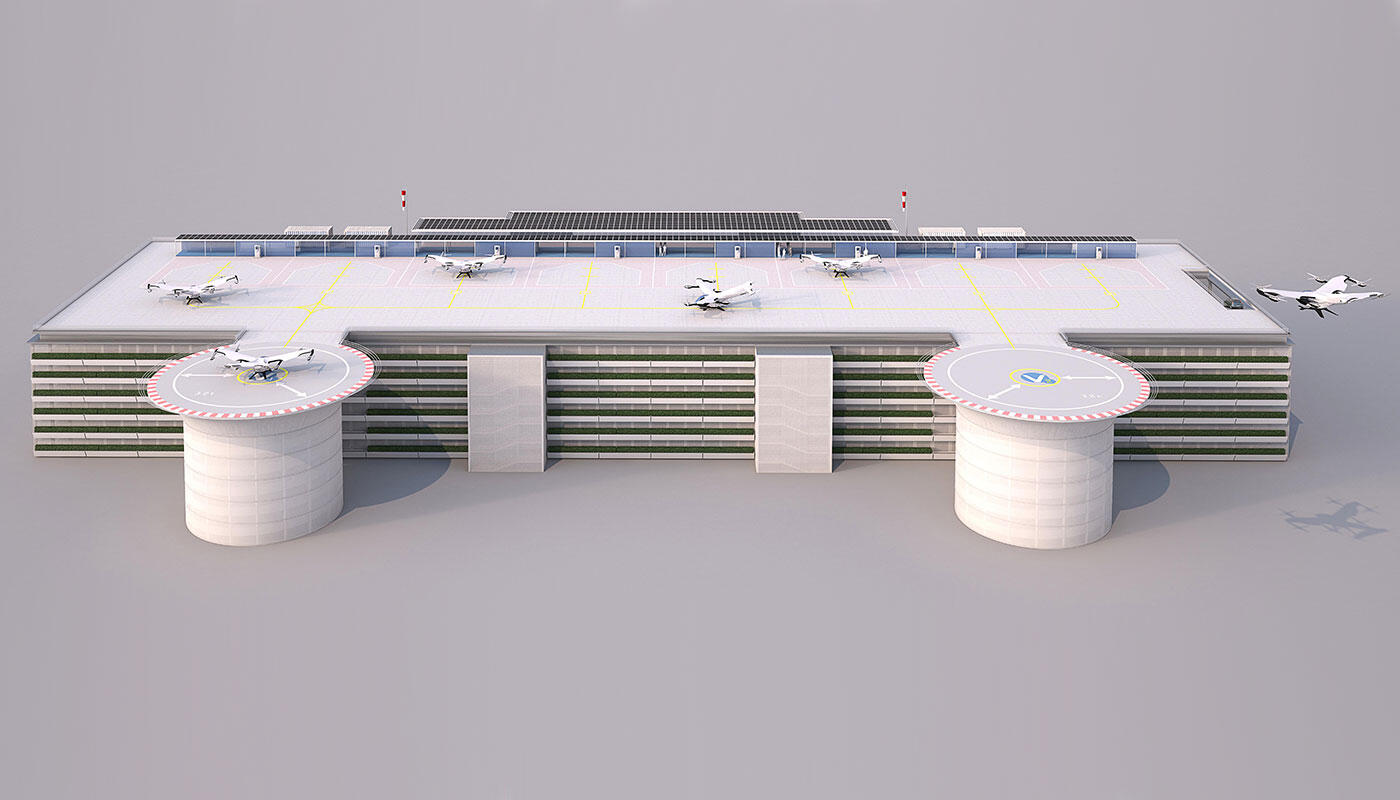
\includegraphics[width=.6\textwidth]{img/vertiport.jpeg}
    \caption{Development of vertiport on a parking garage at \gls{MUC} \cite{amd_vertiport}.}
    \label{vertiport}
\end{figure}